\documentclass[11pt]{article}
\usepackage[letterpaper,margin=1in]{geometry}
\usepackage[T1]{fontenc}
\usepackage[utf8]{inputenc}
\usepackage{lmodern}
\usepackage{amsmath,amssymb}
\usepackage{graphicx}
\usepackage{booktabs}
\usepackage{tabularx}
\usepackage{array}
\usepackage{float}
\usepackage[round,authoryear]{natbib}
\usepackage[hidelinks]{hyperref}

\newcommand{\status}[1]{\textit{#1}}
\newcommand{\obs}{\status{observed}}
\newcommand{\mhr}{\status{modeled}}
\newcommand{\stress}{\status{stress test}}
\newcommand{\hyp}{\status{hypothetical}}
\newcommand{\bp}{\,bp}
\newcommand{\Rsq}{R^2_{\mathrm{OS}}}
\newcolumntype{L}{>{\raggedright\arraybackslash}X}
\renewcommand{\arraystretch}{1.15}
\setlength{\emergencystretch}{2em}
\makeatletter
\renewcommand\section{\@startsection{section}{1}{\z@}{-3.25ex\@plus -1ex \@minus -.2ex}{1.5ex \@plus .2ex}{\normalfont\large\bfseries}}
\renewcommand\subsection{\@startsection{subsection}{2}{\z@}{-3ex\@plus -1ex \@minus -.2ex}{1ex \@plus .2ex}{\normalfont\normalsize\bfseries}}
\long\def\@makecaption#1#2{\vskip\abovecaptionskip\small\textbf{#1.}\ #2\par\vskip\belowcaptionskip}
\setlength{\@fptop}{0pt}
\makeatother

\pagestyle{plain}

\title{\textbf{The Liquidity Paradox}\\[0.5em]
\large Short-horizon predictability, adverse selection and the economics of passive market making:\\
pre-registered evidence from Binance SOLUSDT with a one-time held-out evaluation}
\author{Vatsal Maniar}
\date{November 2026}

\begin{document}
\maketitle

\begin{abstract}
\noindent
Does short-horizon price predictability translate into economically viable passive market making? We reconstruct the
Binance SOLUSDT limit order book on twenty first-of-month sessions and simulate passive execution. Experiments were
specified before their discovery outcomes; a five-session holdout was evaluated once under a protocol frozen in advance.
Liquidity at the best quotes is adversely selected: the 30-second realized spread is $-1.06$\bp{} in discovery and
$-0.59$\bp{} in the holdout. Imbalance forecasts have modest out-of-sample skill ($R^2$ 3.6\% and 4.2\% at five
seconds), yet the forecast-gated rules tested show no material improvement in per-notional fill quality relative to a
placebo. At the only attainable fee tier, every simulated policy that trades loses money in every session; lower
losses come mainly from trading less. Linking adverse selection, forecast skill and costs, we find that
predictability of this size did not make passive quoting profitable here.
\end{abstract}

\noindent\textbf{Keywords:} market making; adverse selection; order-flow imbalance; limit order book; transaction costs;
execution simulation; pre-registration; out-of-sample evaluation; cryptocurrency markets.

\noindent\textbf{JEL classification:} C58, G14, G17.

\section{Introduction}\label{sec:intro}

A large literature shows that the state of a limit order book is informative about very short-horizon price changes.
Order-flow imbalance at the best quotes explains most of the variation in price changes over short intervals
\citep{cont2014}, an imbalance-adjusted micro-price forecasts short-term prices better than the mid \citep{stoikov2018},
and deep networks trained on order-flow histories forecast price moves out of sample, with a relation that is
universal across stocks \citep{sirignano2019} and skill at several short horizons \citep{kolm2023}. A market maker that quotes at the touch might expect to turn such
forecasts into profit by quoting on the side the forecast favours and withdrawing from the side it warns against.

This paper asks whether that expectation survives contact with the mechanics of passive execution. A resting limit
order is filled when someone chooses to trade against it, and that choice is informative. In the canonical information models,
liquidity suppliers lose to better-informed traders and recover the loss from uninformed traders, through the spread
\citep{glosten1985} or through price impact \citep{kyle1985}; the limit order is a free option that informed or faster traders exercise
\citep{copeland1983,foucault2003}. A forecast that moves quotes away from predicted price moves need not remove this
selection: it changes which fills arrive, and the fills that remain are disproportionately those where the forecast was
wrong. Fees,
queue priority and latency then determine whether whatever edge remains is positive after costs.

We study these forces end to end on one market, Binance spot SOLUSDT, using a replay of level-2 book states and the
exchange's trade archive for twenty first-of-month sessions. Four pre-registered experiments build the argument in
order:
\begin{enumerate}
  \item \textbf{E001, observed markouts.} Is liquidity resting at the touch adversely selected, before any modeling of our
  own orders?
  \item \textbf{E002, execution sensitivity.} How much do simulated passive outcomes depend on queue, fill, latency and
  fee assumptions?
  \item \textbf{E003, signals and quoting.} Does out-of-sample forecast skill translate into better fills, and does a
  risk-aware rule improve downside risk?
  \item \textbf{E004, information robustness.} When the participant's market information is delayed or withheld, are
  the fills it receives during staleness worse, and does withdrawing when stale help?
\end{enumerate}

The design was fixed in two stages. Each experiment's specification, with its hypotheses, decision rules and
thresholds, was frozen before that experiment's outcomes on the fifteen discovery sessions were computed. The rules for
the held-out evaluation came later: they were written after the discovery results were known and frozen in a separate
protocol before any outcome on five later sessions, sealed throughout, was computed. Those sessions were then evaluated
once. The protocol defines a test rule for each discovery decision that held. Because five sessions are too
few for interval decisions, every held-out label is a point-estimate check, and the protocol states each check's
evidential weight in advance.

\paragraph{Findings.} Five results organise the paper. Each is labelled by the kind of evidence behind it: \obs,
\mhr, \stress{} or \hyp{} (Section~\ref{sec:evidence}).
\begin{enumerate}
  \item \textbf{Adverse selection at the touch is real and persistent} \obs{}. After an aggressive trade the mid moves
  in the aggressor's direction by about one basis point within a second and keeps drifting for thirty seconds. The
  passive side's realized spread is negative in fourteen or fifteen of fifteen discovery sessions at every primary
  horizon, and in four of five held-out sessions. Its held-out magnitude is 40 to 56\% of the discovery value.
  \item \textbf{Forecast skill is real but small, and the forecast-gated rules tested show no material gain in fill
  quality} (\obs{} forecasts, \mhr{} fills). A linear imbalance model reaches an out-of-sample $R^2$ of 3.6\% in discovery
  and 4.2\% in the holdout at five seconds. Against a placebo that withdraws about as often but in the wrong direction,
  and whose turnover is not matched, the forecast-gated quoter showed no material improvement in per-notional fill
  quality: in discovery the difference lay below the pre-registered 0.5\bp{} margin, and on the holdout it was $-0.01$\bp,
  with a descriptive interval spanning zero. Five held-out sessions cannot establish that the forecast has no economic
  value at all.
  \item \textbf{Fees, not execution assumptions, decide the outcome} \mhr{}. Across three fill models and three latency
  brackets, results differ by less than one basis point; at the attainable 10\bp{} maker fee every policy that trades
  loses about 11 to 12\bp{} of traded notional. No fee schedule we model, including hypothetical rebate tiers, produces a
  positive mean.
  \item \textbf{Lower losses come from trading less} \mhr{}. Every policy that trades loses at a nearly constant rate per
  unit of notional, so hourly losses scale with turnover. The forecast-gated quoter loses about 155\,USDT per hour less than fixed
  quoting in discovery, and 38\,USDT per hour less in the holdout, almost entirely because it trades less: on the
  holdout, 33 of the 38\,USDT is the mechanical saving in maker fees. Abstention is the economically rational decision at
  the attainable fee (a discovery decision; on the holdout the policy results are descriptive, with no confirmation
  claim).
  \item \textbf{Risk controls and information robustness} (\mhr{}, \hyp{}, \stress{}). Inventory skew, withdrawal and a
  volatility gate reduce expected shortfall and drawdown, a result tested (H3) only under a hypothetical rebate tier, and
  they do not produce profit. Under synthetic connection drops, fills arriving while the participant's view was stale showed no material
  deterioration, under a pre-registered 1\bp{} threshold, relative to fills in randomly timed windows of equal duration;
  this is not a finding of equivalence.
\end{enumerate}

\paragraph{Contribution.} The economic forces in this paper are not new: adverse selection, the option value of limit
orders, fee and latency advantages and inventory risk are central to market microstructure, and a recent live
experiment on a Binance perpetual reports that maker fills are negatively selected and that naive top-of-book quoting
loses money even at a rebate tier \citep{albers2025dilemma}. Our results agree with that evidence. What we add is
empirical and methodological. First, we link observed adverse selection, forecast skill, execution assumptions, fees,
inventory controls and information degradation on one spot market, with one replay engine and one set of accounting
identities, so that each stage can be traced to the next. Second, using per-notional contrasts against placebos that withdraw
about as often (in E003, similar quote presence but not similar turnover; in E004, exactly duty-matched windows), we find
that for the forecast-gated rules we tested, the forecast's measurable economic effect came through participation, with
no material improvement in per-notional fill quality, and that comparisons of net profit per hour confound the two.
Third, we report the complete results of a staged pre-registration, in which experiment specifications were fixed before
their discovery outcomes and held-out rules before the one-time held-out evaluation, including the labels that are weak. We do not claim a profitable strategy, and our
negative results concern the fixed, a-priori rules we tested, not every possible quoting policy.

\paragraph{Roadmap.} Section~\ref{sec:lit} reviews related work. Section~\ref{sec:data} describes the data and
sample. Section~\ref{sec:method} sets out the design, the experiments and the inference rules. Section~\ref{sec:results}
reports the results, and Section~\ref{sec:holdout} the held-out evaluation. Section~\ref{sec:discussion} interprets the
evidence, Section~\ref{sec:limits} states its limitations, and Section~\ref{sec:conclusion} concludes. A separate
reproducibility supplement maps every result to the specification and output that produced it.

\section{Related literature}\label{sec:lit}

\paragraph{Adverse selection and inventory.} Two classical channels explain why liquidity suppliers charge a spread.
In information models, a dealer facing traders with private information loses to them on average and sets quotes to
break even against the mixture of informed and uninformed flow, through the spread \citep{glosten1985} or through price
impact \citep{kyle1985}. A resting quote is
equivalent to an option written to the rest of the market \citep{copeland1983}, and in an open limit order book limit
orders earn on small trades while losing on large, informed ones \citep{glosten1994}. Limit-order traders therefore
face two risks: being filled when adverse information arrives, and not being filled when news is favourable
\citep{handa1996}. In inventory models, a dealer shades quotes against its position, to keep inventory within bounds
\citep{amihud1980} or because of risk aversion \citep{ho1981}, and intermediaries' inventories move prices away from fundamental values for hours or days
\citep{hendershott2014}. Spread decompositions separate adverse-selection, inventory and order-processing components
\citep{glosten1988,huang1997}; the information content of a trade can be measured by the persistent price response
that follows it \citep{hasbrouck1991}; and effective and realized spreads, which we use in E001, are standard measures
of execution cost and of the liquidity supplier's revenue net of that response \citep{bessembinder1997}. Textbook
treatments include \citet{ohara1995}, \citet{harris2003}, \citet{hasbrouck2007} and \citet{foucault2013}.

\paragraph{Optimal market making and signals.} Stochastic-control models derive quotes that trade spread capture against
inventory risk, with fills arriving as Poisson processes whose intensity falls with the quote's distance from the mid
\citep{avellaneda2008,gueant2013,cartea2015}. Extensions model how market orders affect future order flow and the
short-term drift, and argue that a quoter that ignores predictors of that drift is adversely selected by better-informed
traders \citep{cartea2014}. \citet{cartea2018} construct a volume-imbalance signal from Nasdaq data, show that it predicts
the sign of the next market order and short-term price moves, and find that incorporating it improves a market-making
strategy calibrated in sample and evaluated on later data. In these models the response of fills to the signal is part
of the model specification. In our replay, which counterparty trades reach the touch comes from the historical stream,
while queue position and fill attribution are modeled and bracketed; this is one plausible reason the two approaches can
differ, which we do not test.

\paragraph{Order-book predictability.} Over short intervals, price changes are explained mainly by order-flow imbalance at
the best quotes, linearly and with a slope inversely related to depth \citep{cont2014}. The micro-price uses spread and
imbalance to forecast the future mid \citep{stoikov2018}. Deep-learning studies find a stable relation between order-flow
history and the direction of the next price move \citep{sirignano2019}, and forecast returns at several horizons from
stationary order-flow features \citep{kolm2023}. Surveys of the empirical regularities of limit order books are given by
\citet{gould2013} and \citet{bouchaud2018}. Our forecasts are deliberately simple, ordinary least squares on eight
decision-time features, because the question is not how much skill can be extracted but whether a known amount of
skill translates into execution value. A small out-of-sample $R^2$ can be economically meaningful for an investor
\citep{campbell2008}; whether it is meaningful for a passive quoter facing fees and selection is the question here.

\paragraph{Liquidity provision, speed and fees.} A case study of a large high-frequency market maker finds that it earns
the spread on mostly passive trades while losing on its inventory positions \citep{menkveld2013}. Across firms, high-frequency
traders' passive trades are adversely selected while their aggressive trades move in the direction of permanent price
changes \citep{brogaard2014}, and relative speed accounts for large differences in trading performance
\citep{baron2019}. Stale quotes are picked off by faster traders, a cost borne by liquidity providers that drives
investment in speed and motivates market-design proposals \citep{foucault2003,budish2015,foucault2017}; in London
equities, latency-arbitrage races cover about a fifth of volume \citep{aquilina2022}. Order flow that adversely selects
market makers has been called toxic, and a volume-based estimate of toxicity (VPIN) has been proposed \citep{easley2012}. The cost of the delay between a decision and
its execution has been modeled \citep{moallemi2013}, and low-latency activity is associated with narrower spreads and
greater depth \citep{hasbrouck2013}. On costs, a simulated trader who knows the future but pays execution costs earns
surprisingly modest profits from aggressive high-frequency strategies \citep{kearns2010}; the split of exchange fees between makers and takers
changes posted quotes and order choice \citep{malinova2015}; and routing limit orders to maximise rebates can worsen their
execution quality \citep{battalio2016}.

\paragraph{Fill modeling and queue position.} With level-2 data, an order's queue position must be inferred. Limit-order
execution times have been modeled econometrically, with the warning that hypothetical executions built from transaction
data are poor proxies for actual executions \citep{lo2002}. Queue-reactive models describe the book as a state-dependent
queuing system and can serve as simulators \citep{huang2015}. Queue position carries value comparable to the spread for
large-tick assets \citep{moallemi2017} and affects an order's adverse-selection risk \citep{garriott2025}, and the interaction
of placement, adverse selection and latency has been modeled directly, with latency reducing the value of imbalance
information \citep{lehalle2017}. We bracket these uncertainties with three fill models and three latency settings rather
than calibrating one, and our simulated orders always join the back of the queue.

\paragraph{Out-of-sample evaluation and research design.} We measure forecast skill with the out-of-sample $R^2$ against a
zero forecast, in the spirit of \citet{campbell2008} and \citet{welch2008}. Concern about data snooping and selective
reporting in empirical finance \citep{white2000,harvey2016,bailey2014,bailey2017} and in science more broadly
\citep{ioannidis2005} motivates our design: each experiment's rules were frozen before its discovery outcomes and the
held-out rules before any held-out outcome, as advocated by the pre-registration literature \citep{nosek2018}, and the
holdout was evaluated once.

\paragraph{Cryptocurrency markets.} Crypto spot and derivatives markets run continuous limit order books with public,
high-frequency data. Prior work documents large and persistent price deviations across exchanges \citep{makarov2020},
evaluates liquidity measures for these markets \citep{brauneis2021}, finds that trade-flow imbalance explains
contemporaneous price changes on a Bitcoin perpetual \citep{silantyev2019}, estimates adverse-selection costs of about a
tenth of the effective spread on one exchange \citep{tinic2023}, and reports moderate predictive power of standard
microstructure measures on Binance, including for SOL \citep{easley2026}. Closest to our question, \citet{albers2025dilemma}
place over two hundred thousand minimum-size maker orders on Binance's Bitcoin perpetual and report that fill probability
and post-fill returns are negatively related, that naive top-of-book quoting is highly unprofitable even at a rebate tier,
and that imbalance-based strategies lose money net of fees; a companion study documents how latency and book updates
make live taker outcomes worse than backtests imply \citep{albers2025latency}. Both are live experiments on crypto derivatives venues (the first
on a Binance perpetual), and the first is a preprint; ours is a pre-registered replay on a spot pair. We regard the agreement between them as more informative than either alone, and we make no claim that the
economic mechanisms differ from those in other markets.

\section{Data and sample}\label{sec:data}

\paragraph{Market and sources.} The instrument is the SOLUSDT spot pair on Binance, quoted on a 0.01\,USDT tick with a
0.001\,SOL lot. Book states come from Tardis's free first-of-month samples of Binance's incremental depth stream, which
we replay into top-ten book states with explicit validity flags. Trades come from Binance's public trade archive, which
carries complete trade identifiers and the exchange's aggressor flag. The recorder's receipt timestamps on Tardis's
trade capture let us know when a trade was \emph{received}, not only when it occurred. Both sources are free; raw files
are kept locally and not redistributed.

\paragraph{Validity.} A data-acceptance test, run before any experiment, rebuilds the book from snapshot anchors and
marks a time interval valid only while the book is provably correct: sequence numbers are continuous, the touch lies
inside the region proven by the last snapshot, the book is uncrossed, and no vendor reconnect intervenes. Invalid
intervals are excluded rather than repaired. An \emph{episode} is an accepted joint (book and trade) window of at
least 600 seconds. Every simulated episode starts flat and ends with all orders cancelled and inventory liquidated
against the visible book.

\paragraph{Sessions and splits.} The sample is twenty first-of-month UTC days (Figure~\ref{fig:design}). The ten
sessions from March to December 2025 form the training split, the five from January to May 2026 the validation split,
and the five from June to October 2026 the held-out test split. Instrument, sample and splits were fixed in October 2026
from data-quality metadata, before any experiment's outcome was computed. That choice was not blind to the test days'
metadata, although their outcomes were sealed (Section~\ref{sec:limits}). E001 and E002 use all fifteen discovery
sessions. E003 and E004 evaluate forecasts and policies walk-forward on sessions six to fifteen, fitting each session's
models only on the sessions before it.

\begin{figure}[t]
  \centering
  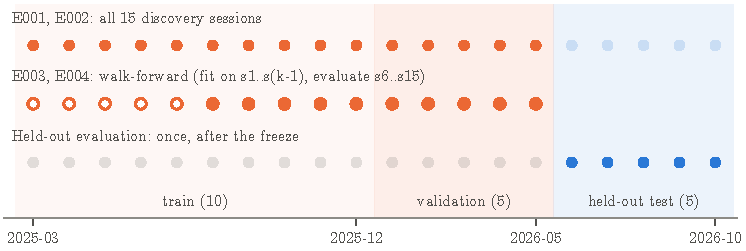
\includegraphics[width=\linewidth]{figures/fig1_design.pdf}
  \caption{Study design. Each dot is one first-of-month session. E001 and E002 use all fifteen discovery sessions. E003
  and E004 evaluate walk-forward: a filled dot is an evaluation session whose models were fitted only on earlier
  sessions; hollow dots are used for fitting only. The five test sessions were sealed until the final protocol was
  frozen and were then evaluated once, with models fitted on all fifteen discovery sessions.}
  \label{fig:design}
\end{figure}

\begin{table}[t]
  \centering\small
  \caption{Sample. Valid hours are the total duration of episodes (accepted joint windows of at least 600\,s).
  Relative tick is the 0.01\,USDT tick as a share of the price. Aggressive events are E001's timestamp-side clusters in
  the primary specification.}
  \label{tab:sample}
  \begin{tabularx}{\linewidth}{L r r r}
    \toprule
    & Discovery (all) & Discovery (walk-forward evaluation) & Held-out test \\
    \midrule
    Sessions & 15 & 10 & 5 \\
    Period & 2025-03 to 2026-05 & 2025-08 to 2026-05 & 2026-06 to 2026-10 \\
    Episodes & 29 & 19 & 20 \\
    Valid hours & 347.5 & 227.9 & 119.7 \\
    Aggressive events (E001) & 4{,}120{,}728 & --- & 720{,}066 \\
    Relative tick (bp) & 0.46--1.20 & --- & 0.85--1.38 \\
    \bottomrule
  \end{tabularx}
\end{table}

Table~\ref{tab:sample} summarises the sample. Two features of the holdout matter later. First, its relative tick is
coarser than in most discovery sessions, because SOL traded at lower prices in 2026; a one-tick spread is therefore
wider in basis points. Second, its valid hours are balanced across sessions (23.7 to 24.0 hours each), but its
episodes are not: 2026-06-01 is split by vendor reconnects into fourteen episodes, while each other session has one or
two. Because each episode restarts flat after a warm-up and ends with a liquidation, 2026-06-01 carries more episode
boundaries than the other four sessions combined.

\section{Methodology}\label{sec:method}

\subsection{Types of evidence}\label{sec:evidence}

The results rest on four kinds of evidence, and each is labelled accordingly. \emph{Observed} results are computed from
recorded exchange trades and replayed book states, with no hypothetical orders. \emph{Modeled} results are historical
replays in which our orders never existed: fills are inferred under stated queue, latency and fee assumptions, and our
orders have no market impact. \emph{Stress-test} results are computed on observed records that were deliberately
degraded. \emph{Hypothetical} marks a fee schedule that a participant like us cannot attain; only the 10\bp{} VIP0
schedule is attainable.

\subsection{Pre-registration and the one-time holdout}\label{sec:prereg}

The order of work was fixed in advance. For each experiment, a written specification was reviewed and fixed before any
outcome of that experiment was computed on market data; the experiment was then run once on the discovery sessions and
analysed with its pre-registered rules. For E003, part of the simulation and feature code was written while the
specification was under review, but no outcome was computed before the specification was fixed. Each later experiment
states the earlier results it could not be blind to and the outcomes those results already suggest, so that a
restatement of known facts is not reported as a discovery. Amendments made after review but before any outcome existed
are dated in the specifications. A pre-registered rule that turned out to be weak was not changed afterwards.

The held-out evaluation was governed by a separate protocol, written after the four discovery experiments and frozen
before the test sessions were opened. Its confirmation rules were therefore written with the discovery results in view:
the experiment specifications fixed the discovery decisions, while the protocol fixed how each decision would be checked
on five sessions, and several of its test forms do not appear in the experiment specifications
(Section~\ref{sec:limits}). What the protocol guarantees is that every held-out rule was fixed before any held-out outcome
was computed. Models fitted on all fifteen discovery sessions were frozen and carried forward without refitting, and
before the evaluation the evaluation code was required to reproduce the frozen discovery results exactly. Each test
session's eligibility was fixed beforehand from data-integrity checks and acceptance metadata that involve no outcomes;
all five sessions were eligible and none was excluded. The protocol also specified in advance how technical failures
would be classified and allowed at most three attempts. The evaluation ran once and completed on its first attempt.

\subsection{Book replay and E001 markouts}\label{sec:e001}

E001 measures what happens after aggressive trades, with no hypothetical orders. An event is a \emph{timestamp-side
cluster}: the exchange trades that share a trade time $T$ and an aggressor side. Binance does not publish parent-order
identifiers, so a cluster is not a verified order, and we report a per-trade specification as a different estimand.
Let $s=+1$ for buyer-initiated and $-1$ for seller-initiated clusters, $P$ the cluster's volume-weighted price, $m_0$ the
mid of the last book state with exchange time before $T$, and $m_{T+h}$ the mid at $T+h$. In basis points of $m_0$,
\begin{equation}
\begin{aligned}
  es &= 2s\,\frac{P-m_0}{m_0}\times 10^4, \qquad mo(h) = s\,\frac{m_{T+h}-m_0}{m_0}\times 10^4,\\
  rs(h) &= es - 2\,mo(h) = 2s\,\frac{P-m_{T+h}}{m_0}\times 10^4 .
\end{aligned}
\end{equation}
The effective spread $es$ is what the aggressor pays relative to the mid, the markout $mo(h)$ is the subsequent mid move
in the aggressor's direction, and the realized spread $rs(h)$ is the liquidity supplier's revenue after that move. The
passive side's mark-to-mid result per unit of liquidity hit is $rs(h)/2$. Primary horizons are 1, 5 and 30\,s; an event
is included only if its pre-event state and every horizon's outcome state lie in the same valid window. The session is
the unit of inference: we report the mean of session means with a 95\% session-bootstrap interval.

\subsection{Execution replay and E002}\label{sec:e002}

The execution engine replays the historical book and trade stream and simulates our orders against it without
altering it: our one-SOL orders have no market impact. The participant decides on the book state it has received, after
a market-data delay; its orders reach the exchange after an entry latency; it learns of fills after an acknowledgement
latency. Orders are post-only at the visible touch, with at most one working order per side. On arrival an order joins
the back of its price level; executions at its price consume the queue ahead of it first. Because level-2 data show
level sizes but not queue positions, the attribution of cancellations is unknown, and we bracket it:
\begin{itemize}
  \item \emph{conservative}: cancellations are assumed to come from behind the order;
  \item \emph{intermediate}: cancellations are credited pro rata to the queue ahead;
  \item \emph{optimistic}: cancellations are credited ahead first, and an order fills when the book moves through it.
\end{itemize}
Three latency brackets cover a Tokyo-hosted setting (2\,ms entry and acknowledgement, no extra data delay), a
regional one (30\,ms each) and a distant one (115\,ms each). Every depth update arrives in the exchange's 100\,ms
batches, so even the fastest bracket decides on batched information. Fees are accounting overlays: the policies in E002
ignore fees, so fills are identical across schedules. Five schedules are modeled (Table~\ref{tab:fees} in
Section~\ref{sec:results}); only VIP0, 10\bp{} maker and 10\bp{} taker, is attainable for this project.

E002 compares two fixed baselines. \textbf{P0} quotes one SOL on both sides at the touch and re-quotes whenever the touch
price changes; a side is posted only if a full fill keeps inventory within $\pm10$\,SOL. \textbf{P1} is P0 that withdraws
the side that would add to inventory once $|q|\ge3$\,SOL. Marked wealth obeys an accounting identity, enforced throughout the
simulation: terminal wealth equals the sum of fill edges against the mid, plus inventory revaluation, minus fees. Results are
liquidation-adjusted. The pre-registered H2 decision asked whether results change sign or ranking across fill-model and
latency scenarios, and whether any paired fill-model difference reaches a materiality threshold of 1.0\bp, about one
tick.

\subsection{Forecasts, quoting policies and E003}\label{sec:e003}

\paragraph{Forecasts.} At each book state $S_k$, the participant's information set contains the state's ten levels per
side, earlier states of the episode and the exchange trades its recorder had received by then. Eight features are
computed from this set: touch imbalance, five-level imbalance, best-level order-flow imbalance over one and ten seconds
\citep{cont2014}, signed trade flow over one and ten seconds, the ten-second return and the spread. The target is the
log change, in basis points, from the mid of $S_k$ to the mid $h$ seconds after the regional decision time (receipt of
$S_k$ plus 30\,ms); the primary horizon is five seconds. Model M1 regresses
the target on touch imbalance alone; M2 uses all eight features. Both are fitted by ordinary least squares on every fifth
eligible state of the training sessions, with sessions weighted equally and regressors clipped at training quantiles.
There is no regularisation, model search or non-linear model. Skill is the out-of-sample $R^2$ against the zero forecast,
\begin{equation}
  \Rsq = 1 - \frac{\sum_k (y_k - \hat f_k)^2}{\sum_k y_k^2},
\end{equation}
computed per evaluation session and averaged.

\paragraph{Policies.} All policies post one SOL at the touch or not at all, keep a working order at the wanted price (so
it retains its queue position), respect the $\pm10$\,SOL limit and draw new orders from a token bucket of 1.15 orders per
second per side. With $s$ the spread in ticks, $f$ the forecast converted to ticks, $c$ the maker fee in ticks and $q$
inventory, the rules are summarised in Table~\ref{tab:policies}. At VIP0 the maker fee is about 8 to 17 ticks at the
evaluation sessions' prices, against a mean absolute five-second forecast of about half a basis point, roughly one tick
or less.

\begin{table}[t]
  \centering\small
  \caption{Quoting policies (E003). All quote one SOL at the touch. Fee-unaware policies are simulated once and fees
  are overlaid; P3F and P4 depend on the maker fee and are simulated per schedule.}
  \label{tab:policies}
  \begin{tabularx}{\linewidth}{l L L}
    \toprule
    Policy & Quote the bid when & Role \\
    \midrule
    NT & never & no-trade baseline \\
    P0 & always & fixed quoting (E002) \\
    P1 & $q<3$ (the ask mirrors) & inventory withdrawal (E002) \\
    P3[M] & $s/2 + f > 0$ (ask: $s/2 - f > 0$) & forecast-gated, fee-unaware; M $\in\{$M1, M2$\}$ \\
    P3[$-$M2] & $s/2 - f > 0$ (ask: $s/2 + f > 0$) & placebo: same gate, wrong direction \\
    P3F & $s/2 + f - c > 0$ & forecast- and fee-aware \\
    P4 & P3F's condition with $f-\kappa q$, $q<3$, volatility gate open & P3F plus inventory skew ($\kappa=0.25$ tick/SOL), withdrawal and a volatility gate \\
    \bottomrule
  \end{tabularx}
\end{table}

\paragraph{Pre-registered decisions.} E003 fixed three primary decisions, evaluated on the walk-forward sessions under
the primary execution scenario (intermediate fill model, regional latency):
\begin{itemize}
  \item \textbf{H1-F, forecast skill:} the 95\% session-bootstrap interval of M2's session-mean $\Rsq$ at five seconds
  lies above zero.
  \item \textbf{H1-T, translation:} $D$ = gross (pre-fee) basis points of traded notional of P3[M2] minus those of the
  placebo P3[$-$M2], with margin $\delta=0.5$\bp. The placebo withdraws about as often (two-sided quote presence 35\%
  against 31\%) but in the wrong direction; its turnover is not matched, so $D$ compares fill quality per unit of
  notional. Fees are a constant rate on notional and cancel to first order.
  The project's hypothesis H1 states that better prediction does not necessarily imply better after-cost outcomes, so
  \emph{H1 supported} means skill without material translation; it requires H1-F and an upper bound of $D$ below $\delta$.
  \item \textbf{H3, risk components:} P4 minus P3F under the hypothetical LP tier 4 schedule, where both trade. H3 is
  supported if the intervals of the differences in expected shortfall of five-minute P\&L increments and in maximum
  drawdown both lie below zero, and the lower bound of the net-per-hour difference lies above $-\delta_h$, with
  $\delta_h$ equal to 10\% of the comparator's absolute mean.
\end{itemize}
A separate participation decision prefers a policy to not trading only if its net-per-hour interval,
Bonferroni-adjusted over the seven candidate policies (P0, P1, P3[M1], P3[M2], P3[$-$M2], P3F and P4), lies above zero.

\subsection{Information degradation and E004}\label{sec:e004}

E004 asks what happens when the participant's information degrades while the market does not. Degradations are applied
to the participant's view only; the exchange-side event stream, queue estimates and fills are bit-identical across
conditions. The primary cell, D1-E, simulates connection drops: book states and trades delivered during a drop are lost,
and a full book is re-delivered on resume. Drops arrive as a Poisson process at 120 per hour, with durations drawn from
the six reconnect gaps observed in discovery; about 4.5\% of time is stalled. The rate is a stress level, about 7{,}000
times the observed reconnect rate. Secondary cells simulate book-feed stalls with trades continuing (D1-S), delayed
rather than lost records (D3), trade-feed outages (D2, a negative control) and noise in displayed sizes (D4). Degradation
schedules are generated from fixed seeds and were fixed before any E004 outcome was computed.

\paragraph{Primary contrast.} Within a single run of the naive policy (which keeps quoting on stale states), let
$W_U$ be the time during which the participant's information age is at least $\tau=650$\,ms, and $W_P$ a placebo set of
windows with exactly the same total duration and spell lengths, shifted to random times. For a window set $W$,
$q(W)$ is the fee-free five-second mark-to-mid of fills inside it, in basis points of their notional. The contrast is
\begin{equation}
  D_W = q(W_P) - q(W_U),
\end{equation}
positive when fills during staleness are worse than fills at random times. H4-W asks whether $D_W$ exceeds $\delta=1$\bp,
for two bases, P0 and P3[M2]. The label \emph{immaterial selection} requires an upper bound below $\delta$. The contrast is
fee-free, involves no path divergence between arms, and is matched exactly on withdrawal duty; fills and turnover are not
matched, so it compares quality per unit of notional rather than totals and is free of the participation confound that
affects net-per-hour comparisons.

\paragraph{Secondary contrasts.} At the forecast level, staleness-aware shrinkage of the forecast is compared with the
naive forecast and a placebo shrinkage. With $L$ the skill lost to degradation and $A$ the part recovered by shrinkage,
the recovered share is $\rho_A=\sum A/\sum L$. The specification projected in advance, from E003's results, that this
share would be about 0.37 for the true current mid ($y_k$) and about zero for the mid the participant actually prices
against ($y_\mathrm{view}$); the latter projection makes the $y_\mathrm{view}$ result largely implied by the choice of
target.

\subsection{Inference and the held-out labels}\label{sec:inference}

On discovery sessions the session is the unit: means of session values, paired differences on the same sessions, and
10{,}000-draw session-bootstrap percentile intervals \citep{efron1993}. For E003 and E004, the number of sessions of each
sign is reported beside every interval, and Bonferroni-adjusted intervals over each primary family are reported; they
change no label. E001's intervals are unadjusted, and E002's H2 rule uses no multiplicity adjustment.

On the five held-out sessions the protocol makes no interval decision. Each primary discovery decision that held, and
the secondary $y_\mathrm{view}$ decision, has a test rule (Table~\ref{tab:holdout}): a check that the mean has the
discovery sign or lies on the discovery side of its threshold (for $y_\mathrm{view}$, that the ratio $\rho_A$ does);
E001's rule and E004's H4-W rule add a four-of-five count condition, and H3 adds the non-inferiority margin. E002, H4-0
(reported only under E004's specification), the VIP0 participation decision (no rule on test) and the decisions that were
inconclusive or not testable in discovery are reported only (Table~\ref{tab:reported}). E001 had no confirmation rule in
discovery; the final protocol added one. A rule that is met is labelled \emph{confirmed (point estimate)}; otherwise \emph{not
confirmed}, which on five sessions is not a refutation. Descriptive $t$-intervals are printed beside test values but
are not used for any label. The protocol also states the evidential weight of each rule in advance: a rule decided by
the sign of a mean alone, as E003's three are, could be met with probability up to one half under a null distribution
symmetric about its threshold; a single four-of-five count condition has probability 6/32, or 18.75\%, under
independent sessions and a null whose median sits at the threshold. Confirmations are tallied per experiment; a tally is
not a count of independent replications.

\section{Results}\label{sec:results}

We present each experiment's discovery result and its held-out counterpart together. Section~\ref{sec:holdout} then
assembles the held-out labels.

\subsection{Liquidity at the touch is adversely selected}\label{sec:res-e001}

Over 4.12 million aggressive clusters in fifteen discovery sessions, aggressors paid an effective spread of $+1.28$\bp{}
[1.13, 1.43] \obs{}. The mid then moved in their direction: $+0.99$\bp{} after one second and $+1.17$\bp{} after thirty
(Figure~\ref{fig:markouts}). The realized spread was $-0.69$\bp{} at one second and $-1.06$\bp{} [$-1.24$, $-0.86$] at
thirty, negative in fourteen, fourteen and fifteen of fifteen sessions at the three primary horizons. Per unit of
liquidity hit, the passive side's mark-to-mid loss at thirty seconds was $0.53$\bp{} per cluster and, in an exploratory
quantity-weighted view (discovery only), $1.10$\bp{} per unit of traded quantity, before fees, against a one-tick spread of 0.46 to 1.20\bp.

\begin{figure}[t]
  \centering
  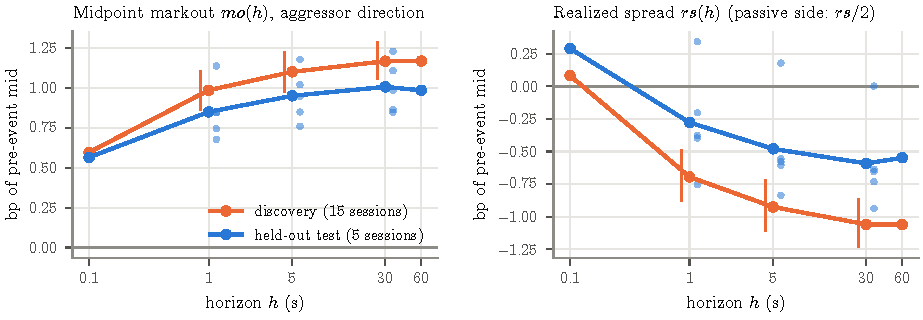
\includegraphics[width=\linewidth]{figures/fig2_markouts.pdf}
  \caption{Post-trade markouts \obs{}. Left: the mid move in the aggressor's direction. Right: the realized spread, the
  liquidity supplier's revenue after that move. Lines are means of session means; orange bars are discovery 95\%
  session-bootstrap intervals at the primary horizons; blue dots are individual held-out sessions. The 0.1\,s and 60\,s
  horizons are declared secondary horizons, reported descriptively.}
  \label{fig:markouts}
\end{figure}

The timing matters. In exploratory addenda declared before computation and not computed on the holdout, about
0.65\bp{} of the 1.17\bp{} thirty-second markout occurs within the 100\,ms depth batch that contains the trade, and the
pooled passive result is close to zero at 100\,ms before turning negative. This pooled average mixes
two profiles: in the 49\% of clusters whose hit-side touch price changed within the batch, the passive side is behind at
once; where the touch stayed, it starts slightly favourable and decays to about zero. Imbalance cells conditioned on
the realized trade direction show the same pattern, but they condition on information a quoter does not have when it
posts, so we treat them as description and leave the decision-time question to E003.

On the holdout, the pattern holds with a smaller magnitude. Markouts were positive in all five sessions at every primary
horizon, with means of $+0.85$, $+0.95$ and $+1.01$\bp{}, about 86\% of their discovery values. Realized spreads were
negative in four of five sessions, with means of $-0.28$, $-0.48$ and $-0.59$\bp{}, 40 to 56\% of the discovery values.
The exception is 2026-08-01, whose realized spreads were positive at one and five seconds and essentially zero at thirty
($+0.002$\bp, counted as positive). The
descriptive $t$-interval for the one-second realized spread, $[-0.77, +0.22]$, includes zero. The pre-event book state
was also older in the holdout (90th percentile 137\,ms against 95\,ms in discovery), a descriptive difference we do
not interpret further.

\subsection{Fees, not execution assumptions, decide the outcome}\label{sec:res-e002}

Across six combinations of policy and fill model and three latency brackets, the session-mean net result of P0 and P1 at
VIP0 lay between $-11.07$ and $-11.87$\bp{} of traded notional in discovery \mhr{}, with every bootstrap interval far
below zero and every session negative. The pre-registered H2 decision was \emph{not supported}: no scenario reversed a
sign or a ranking, and no paired fill-model difference was material (0.16 to 0.55\bp, all below the 1.0\bp{} threshold,
though all intervals excluded zero). Lower latency produced more fills and slightly worse results per unit of notional:
the fills it adds are more adverse.

The loss decomposes cleanly. Before fees, the policies lost 1.1 to 1.9\bp{} of notional: spread capture against the mid
before the fill was only $+0.2$ to $+0.4$\bp, while inventory revaluation cost $1.5$ to $2.2$\bp. Our own fills' thirty-second
markouts ($-1.1$ to $-1.9$\bp) match E001's exploratory $-1.10$\bp{} per unit of hit volume: the simulated fills are adversely
selected about as much as the average liquidity at the touch. The fee then adds about 10\bp. Table~\ref{tab:fees} and
Figure~\ref{fig:fees} show how the result moves with the fee schedule while fills are held fixed. No schedule, including
the hypothetical LP tier 4 rebate of 0.8\bp, produces a positive mean.

\begin{table}[t]
  \centering\small
  \caption{Fee schedules (E002, discovery). Net results for P0 at Tokyo-hosted latency span the three fill models. Fills
  are identical across schedules; only the fee overlay changes. LP-programme taker rates are assumed equal to VIP9's.}
  \label{tab:fees}
  \begin{tabular}{l r r l r}
    \toprule
    Schedule & Maker (bp) & Taker (bp) & Status & Net (bp of notional) \\
    \midrule
    VIP0 & 10.0 & 10.0 & attainable & $-11.9$ to $-11.4$ \\
    VIP0 + BNB & 7.5 & 7.5 & \hyp & $-9.4$ to $-8.9$ \\
    VIP9 & 1.1 & 2.3 & \hyp & $-3.0$ to $-2.5$ \\
    LP tier 1 & 0.0 & 2.3 & \hyp & $-1.9$ to $-1.4$ \\
    LP tier 4 & $-0.8$ & 2.3 & \hyp & $-1.1$ to $-0.6$ \\
    \bottomrule
  \end{tabular}
\end{table}

\begin{figure}[t]
  \centering
  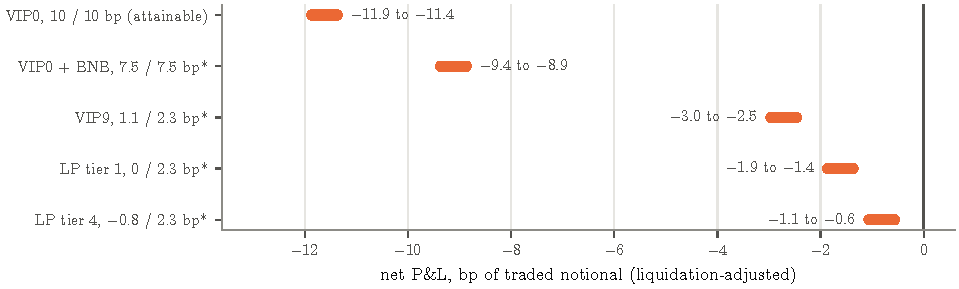
\includegraphics[width=\linewidth]{figures/fig3_fees.pdf}
  \caption{Net result by fee schedule \mhr{}, discovery sessions, policy P0, Tokyo-hosted latency. Each bar spans the
  session-mean results of the conservative, intermediate and optimistic fill models. Starred schedules are
  \hyp{}.}
  \label{fig:fees}
\end{figure}

E002 made no confirmation claim on the holdout: because H2 was not supported in discovery, its frozen specification
requires only that the same tables be reported. They are consistent with discovery. At VIP0 the eighteen scenario means
lay between $-10.99$ and $-11.95$\bp{} of notional, and the range across fill models at fixed policy and latency was 0.59
to 0.67\bp{} (descriptive; materiality is not assessed on the holdout), against 0.49 to 0.55\bp{} in discovery.

\subsection{Predictability without translation}\label{sec:res-e003}

\paragraph{Skill.} The eight-feature model M2 had out-of-sample skill at every horizon \obs{}: an $\Rsq$ of 4.1, 3.6 and
1.4\% at one, five and thirty seconds in discovery, positive in all ten walk-forward sessions at five seconds, with an
information coefficient of 0.21 and a sign hit rate of 65\%. Touch imbalance alone (M1) achieved 3.5\%; the other seven
features added 0.13 percentage points, an increment whose interval included zero. In the holdout, with models fitted on
all fifteen discovery sessions, M2's five-second $\Rsq$ was 4.2\% (positive in all five sessions, ranging from 1.4 to
6.0\%), its information coefficient again 0.21 and its hit rate 66\%. By horizon, it reached 5.7, 4.2 and 1.4\%.

\paragraph{Translation.} The forecast-gated rule showed no material improvement in fill quality. In discovery, the forecast-gated quoter P3[M2] and its
placebo P3[$-$M2] differed by $D=-0.12$\bp{} [$-0.32$, $+0.07$] in gross basis points of notional \mhr{}, with P3[M2]
\emph{worse} in six of ten sessions; the pre-registered label was \emph{H1 supported}: skill without material translation.
The mechanism is selection conditional on being filled. P3[M2] withdraws the side its forecast warns against, so the
fills it still receives are disproportionately those where the forecast was wrong. Its own five-second fill markout was
$-1.72$\bp, against $-1.37$\bp{} for fixed quoting. In the holdout, $D$ was $-0.01$\bp: negative, as in discovery, but by a
margin of one hundredth of a basis point, with two of five sessions negative, one session at $+0.50$\bp, and a
descriptive interval of $[-0.48, +0.46]$. Under the frozen rule this is \emph{confirmed (point estimate)}; in substance
it says only that, in the holdout too, the forecast-gated rule showed no material per-notional improvement over a placebo
whose turnover was not matched. With an interval spanning zero and five sessions, it cannot establish that no improvement
exists. It is the weakest label in the evaluation.

\begin{table}[t]
  \centering\small
  \caption{Quoting policies at the attainable fee (VIP0) \mhr{}. Primary scenario: intermediate fill model, regional
  latency. Means over the ten walk-forward discovery sessions and the five held-out sessions. Turnover is traded notional
  per valid hour. Every policy that traded lost money in every session of both samples; P3F and P4 abstained. The
  held-out columns are descriptive, with no test rule.}
  \label{tab:policies-results}
  \setlength{\tabcolsep}{3.5pt}
  \begin{tabular}{l r r r r r}
    \toprule
    & \multicolumn{2}{c}{Discovery} & \multicolumn{3}{c}{Held-out test} \\
    \cmidrule(lr){2-3}\cmidrule(lr){4-6}
    Policy & Turnover (USDT/h) & Net (USDT/h) & Turnover (USDT/h) & Gross (USDT/h) & Net (USDT/h) \\
    \midrule
    P0 & 171{,}157 & $-197.4$ & 54{,}557 & $-7.7$ & $-62.3$ \\
    P1 & 148{,}486 & $-171.0$ & 48{,}159 & $-6.8$ & $-55.0$ \\
    P3[M1] & 35{,}805 & $-42.1$ & 21{,}255 & $-3.4$ & $-24.7$ \\
    P3[M2] & 35{,}692 & $-42.3$ & 21{,}379 & $-3.3$ & $-24.8$ \\
    P3[$-$M2] & 158{,}228 & $-183.6$ & 51{,}111 & $-7.5$ & $-58.7$ \\
    P3F, P4 & 0 & 0.0 & 0 & 0.0 & 0.0 \\
    No trade & 0 & 0.0 & 0 & 0.0 & 0.0 \\
    \bottomrule
  \end{tabular}
\end{table}

\subsection{Lower losses come from trading less}\label{sec:res-participation}

Table~\ref{tab:policies-results} and Figure~\ref{fig:turnover} show the economic outcome at VIP0. Every policy that
traded lost money in every session of both samples, and every policy lies close to a single line through the origin: net
profit per hour is roughly turnover times a constant loss of 11 to 12\bp{} of notional. The ranking of policies by
hourly loss is therefore, to first order, a ranking by how much they trade.

\begin{figure}[t]
  \centering
  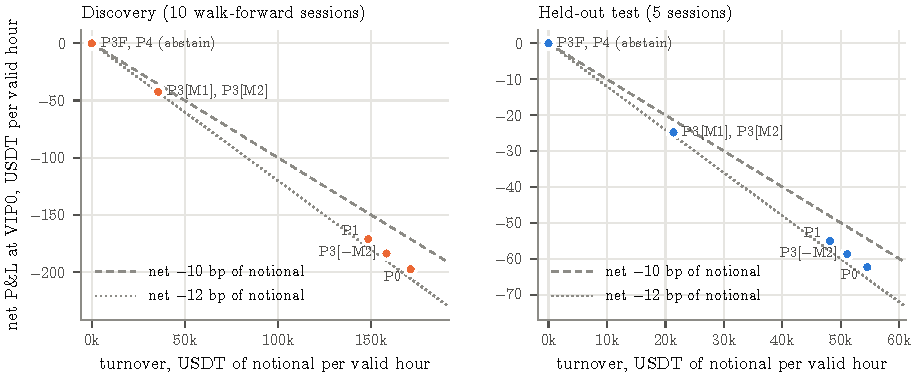
\includegraphics[width=\linewidth]{figures/fig4_turnover.pdf}
  \caption{Net profit per hour against turnover at VIP0 \mhr{}, primary scenario. Points are reported policy means;
  P3[M1] and P3[M2] overlap. Reference lines mark a constant net loss of 10 and 12\bp{} of traded notional. Every policy
  that trades lies on or between them, so lower hourly losses come with lower turnover. The fee-aware policies abstain and sit
  at the origin, with the no-trade baseline.}
  \label{fig:turnover}
\end{figure}

This is the sense in which the forecast has economic value. In discovery P3[M2] lost $155$\,USDT per hour less than P0
[84, 234], in all ten sessions, because it avoided about 79\% of P0's fills, which on average lost money. The placebo,
whose quote presence was similar (35\% against 31\% two-sided) but whose turnover was more than four times larger, lost
almost as much as P0: it keeps exactly the quote that the coming move will fill. In the holdout P3[M2] lost $37.5$\,USDT
per hour less than P0, in all five sessions. Of that difference, $33.2$\,USDT per hour is the maker fee P3[M2] did not pay
on the notional it did not trade, and $4.4$\,USDT per hour comes from gross trading results. Per unit of notional,
P3[M2]'s gross result was 0.05\bp{} \emph{worse} than P0's.

Lower losses per hour therefore do not establish predictive trading alpha. A rule that trades less loses less when every
unit of trading loses; the comparison that addresses fill quality is the per-notional placebo contrast $D$, which showed
no material improvement (an upper bound below 0.5\bp{} in discovery, $-0.01$\bp{} in the holdout), although the placebo
was not matched on turnover. The pre-registered participation decision reflects this: no candidate policy's
net-per-hour interval lay above zero in discovery, and the fee-aware policies, whose gates compare the forecast with the
fee, never traded. On the holdout this decision has no test rule; the policy results there are descriptive, with no
confirmation claim. A 10\bp{} maker fee is 8 to 17 ticks at these prices; a forecast averaging half a basis point cannot clear it.
\emph{At the attainable fee, the economically rational decision for these policies is not to participate.}

The hypothetical schedules do not change this conclusion. Under VIP9, P3F and P4 traded 9\% and 7\% of P3[M2]'s notional in
discovery and still lost; under the LP tier 4 rebate every policy still lost on average, the smallest loss being P3[M1]'s
$3.4$\,USDT per hour.

\subsection{Risk controls reduce risk, not losses}\label{sec:res-h3}

Under the hypothetical LP tier 4 schedule, where the fee-aware policies trade, P4 differs from P3F only in its risk
components: inventory skew, withdrawal at three SOL and a volatility gate. In discovery P4 cut time-averaged absolute
inventory by about two thirds (1.8 against 5.5\,SOL), lowered the expected shortfall of five-minute increments by $3.9$\,USDT [$-5.4$, $-2.6$]
and maximum drawdown by 69\,USDT [$-108$, $-38$], and lost $3.0$\,USDT per hour less [1.6, 4.6] \mhr, \hyp. Its turnover
was 78\% of P3F's, so the reduction was not labelled mechanical, and the reductions held per unit of turnover. H3 was
supported.

The holdout reproduced every sign. Expected shortfall fell by $1.87$\,USDT and drawdown by $19.0$\,USDT, in all five
sessions, and net profit per hour rose by $0.65$\,USDT, also in all five, above the non-inferiority margin of $-1.18$. The
label is \emph{confirmed (point estimate)}. Three qualifications bound it. First, it holds only under a fee schedule that
is not attainable. Second, the net improvement shrank to about a fifth of its discovery size. Third, both policies still
lose under that schedule, and a turnover ratio above the pre-registered 0.50 threshold for a \emph{partly mechanical}
label (0.78 in discovery, 0.82 in the holdout) does not show that the risk reduction is independent of activity. The
improvement is also relative to P3F only: under the same hypothetical schedule the fee-unaware P3[M2] lost less per hour
than P4 ($-3.7$ against $-8.8$\,USDT in discovery; $-1.6$ against $-2.7$ in the holdout, descriptive). In the holdout under
VIP9 (descriptive) the same signs appeared on ES and drawdown, but both policies traded under 5\% of P3[M2]'s notional (9\%
and 7\% in discovery). Risk controls reduced the variability and depth of losses; they did not create profit.

\subsection{Stale information: no material deterioration in fill quality}\label{sec:res-e004}

E004's specification expected stale information to hurt mechanically: orders left resting at stale prices should be
filled by trades that run through them. The data showed no material deterioration under the 1\bp{} threshold
\mhr, \stress. In discovery, $D_W$ was $-0.04$\bp{}
[$-0.11$, $+0.02$] for P0 and $-0.16$\bp{} [$-0.30$, $+0.003$] for P3[M2], below the 1\bp{} margin in all ten sessions; both
labels were \emph{immaterial selection}. The point estimates were slightly negative, that is, fills during staleness
were if anything slightly better than fills at random times. P0 was filled less often in stale windows, because quotes
left behind by a move are not filled while quotes the move runs into are, with no material deterioration in quality per
unit of notional. In the holdout, $D_W$ was $-0.09$\bp{} for P0 and $-0.08$\bp{}
for P3[M2], below the margin in all five sessions and negative in three of five for each; both labels are
\emph{confirmed (point estimate)}, and a stall-only qualifier gives the same result. Under the protocol's required
wording, these are findings of \emph{no material deterioration under the specified threshold}: they are not
equivalence, and they say nothing about effects smaller than one basis point.

The realised comparison of withdrawing when stale against withdrawing at random times, matched on participation, showed
no gain from timing withdrawal by staleness in either sample (descriptive). Every net gain from withdrawing at all came
almost entirely from the mechanical fee saving on lower turnover, the same participation effect as in E003. Withdrawing
at all, whether when stale or at random, slightly worsened fills per unit of notional relative to never withdrawing
(descriptive), consistent with models in which queue position affects adverse-selection risk
\citep{moallemi2017,garriott2025}; we did not test whether re-posting is the mechanism. At the forecast level
(\stress), staleness-aware shrinkage recovered part of the skill lost against the true current mid (held-out
$\rho_A=0.36$, against a projection of 0.37; discovery label \emph{inconclusive}, reported only) and essentially none
against the mid the participant prices from: the secondary $y_\mathrm{view}$ row, $\rho_A=0.011$ against a projection of
zero, is \emph{confirmed (point estimate)} as \emph{not supported}, an outcome largely implied by the choice of target. On
clean data (H4-0, \obs{} with a model trained under \stress), the shrunk forecast's skill differed from the reference by $+0.03$ percentage points in discovery (labelled
\emph{harmless}) and by $+0.001$ in the holdout (reported only).

\section{The held-out evaluation}\label{sec:holdout}

Tables~\ref{tab:holdout} and~\ref{tab:reported} together reproduce the full per-experiment label table: every
pre-registered decision with its discovery result, its frozen test rule where it has one, and its held-out value;
Figure~\ref{fig:holdout} plots a selection. Per experiment,
the tallies were E001 6 of 6, E003 3 of 3 and E004 (H4-W) 2 of 2 confirmed (point estimate); the secondary
$y_\mathrm{view}$ row, outside the tally, was also confirmed (point estimate). No session was undefined, no experiment
failed, and no check was flagged.

\begin{table}[p]
  \centering\footnotesize
  \setlength{\tabcolsep}{3.5pt}
  \newcommand{\grp}[1]{\multicolumn{5}{>{\raggedright\arraybackslash}p{\dimexpr\linewidth-2\tabcolsep\relax}}{#1}}
  \caption{The held-out evaluation: confirmatory checks. Discovery values are means of session values with 95\%
  session-bootstrap intervals and sign counts. Test rules were frozen before the holdout was opened. ``c.p.e.''
  abbreviates the frozen label \emph{confirmed (point estimate, 5 of 5 defined)}. Every label is a point-estimate check on
  five sessions, not a test of statistical significance; descriptive $t$-intervals, which the protocol does not use, are
  given for the weakest checks. Tallies are per experiment and are not counts of independent replications. Items without
  a test rule are in Table~\ref{tab:reported}.}
  \label{tab:holdout}
  \begin{tabularx}{\linewidth}{>{\raggedright\arraybackslash}p{2.2cm} >{\raggedright\arraybackslash}p{3.15cm} >{\raggedright\arraybackslash}p{2.85cm} >{\raggedright\arraybackslash}p{2.5cm} L}
    \toprule
    Check (status) & Discovery & Frozen test rule & Held-out test & Label and comment \\
    \midrule
    \grp{\textbf{E001, observed markouts} (\obs). Tally: \textbf{6 of 6 confirmed}. One family linked by $rs=es-2mo$; rule added by the final protocol.} \\
    $mo$ 1 / 5 / 30\,s & $+0.99$ / $+1.10$ / $+1.17$\bp; 15/15 positive & mean has the discovery sign, which holds in $\ge4$ of 5 sessions & $+0.85$ / $+0.95$ / $+1.01$; 5/5 positive & c.p.e.\ $\times3$; about 86\% of discovery size \\
    $rs$ 1\,s & $-0.69$ [$-0.88$, $-0.48$]; 14/15 negative & same & $-0.28$; 4/5 negative & c.p.e.; $t$-interval $[-0.77, +0.22]$ includes zero \\
    $rs$ 5 / 30\,s & $-0.93$ / $-1.06$; 14/15 and 15/15 negative & same & $-0.48$ / $-0.59$; 4/5 negative & c.p.e.\ $\times2$; 52 and 56\% of discovery size \\
    \addlinespace
    \grp{\textbf{E002, execution sensitivity} (\mhr). No confirmatory check: H2 was not supported in discovery (Table~\ref{tab:reported}).} \\
    \addlinespace
    \grp{\textbf{E003, signals and quoting}. Tally: \textbf{3 of 3 confirmed}.} \\
    H1-F (\obs) & $\Rsq$ 3.64\% [2.97, 4.35]; 10/10; \emph{holds} & mean $\Rsq>0$ & 4.20\%; 5/5 positive & c.p.e.; sign of a mean only \\
    H1-T (\mhr, gross) & $D=-0.12$ [$-0.32$, $+0.07$]; 4/10 positive; \emph{H1 supported} & mean $D<0$ and $<\delta=0.5$\bp & $-0.01$; 2/5 negative & c.p.e.\ by a margin of 0.01\bp; $t$-interval $[-0.48, +0.46]$; weakest label \\
    H3 (\mhr, \hyp{} LP tier 4) & ES $-3.9$, drawdown $-69$, net/h $+3.0$\,USDT; \emph{H3 supported} & each difference has the discovery sign; net/h $>-\delta_h=-1.18$ & ES $-1.87$, drawdown $-19.0$, net/h $+0.65$; 5/5 each & c.p.e.; hypothetical fees; net gain about a fifth of discovery \\
    \addlinespace
    \grp{\textbf{E004, information robustness}. Tally (H4-W): \textbf{2 of 2 confirmed}; the $y_\mathrm{view}$ row is secondary and outside the tally.} \\
    H4-W[P0] (\mhr{} under \stress) & $D_W=-0.04$ [$-0.11$, $+0.02$]; \emph{immaterial selection} & mean $D_W<1$\bp{} and $<1$\bp{} in $\ge4$ of 5 & $-0.09$; 5/5 below 1\bp; 3/5 negative & c.p.e.: no material deterioration under the specified threshold \\
    H4-W[P3[M2]] (\mhr{} under \stress) & $D_W=-0.16$ [$-0.30$, $+0.003$]; \emph{immaterial selection} & same & $-0.08$; 5/5 below 1\bp; 3/5 negative & c.p.e., as above \\
    H4-F $y_\mathrm{view}$, D1-S and D3 (\stress; secondary) & $\rho_A=-0.007$, $-0.008$; \emph{not supported} & $\rho_A<0.25$ & $0.011$, $0.011$ & c.p.e.: \emph{not supported} holds; largely implied by the target choice \\
    \bottomrule
  \end{tabularx}
\end{table}

\begin{table}[t]
  \centering\footnotesize
  \setlength{\tabcolsep}{3.5pt}
  \caption{The held-out evaluation: items reported only. These discovery decisions have no test rule (they were not
  supported, inconclusive, not testable or descriptive in discovery, or the frozen specification makes them reported
  only), so no confirmation claim is made; the held-out values are descriptive.}
  \label{tab:reported}
  \begin{tabularx}{\linewidth}{>{\raggedright\arraybackslash}p{3.0cm} >{\raggedright\arraybackslash}p{4.3cm} >{\raggedright\arraybackslash}p{3.6cm} L}
    \toprule
    Item (status) & Discovery & Held-out test & Comment \\
    \midrule
    E001 $es$ (\obs) & $+1.28$\bp{} [1.13, 1.43]; 15/15 positive & $+1.42$; 5/5 positive & close to mechanical; no confirmatory weight \\
    E002 H2 (\mhr) & \emph{not supported}: no sign or ranking reversal; fill-model differences 0.16--0.55\bp & VIP0 means $-10.99$ to $-11.95$\bp & no confirmation claim (E002 \S10.10) \\
    E003 participation at VIP0 (\mhr) & no policy's interval above zero; \emph{abstention rational} & every policy that trades lost in 5/5 sessions; P3F and P4 abstained & descriptive \\
    E004 H4-F $y_k$, D1-S and D3 (\stress) & $\rho_A=0.57$; \emph{inconclusive} & $\rho_A=0.36$, $0.36$ (projection 0.37) & reported against the projection \\
    E004 H4-F, D1-E, D2, D4 (\stress) & \emph{not testable}; \emph{not testable} (negative control); \emph{inconclusive} & D1-E and D2 below the skill-loss gate; D4 $\rho_A=0.18$ & no \emph{pending review} flag \\
    E004 H4-F D1-S1, D1-S3 (\stress; dose-response) & descriptive, no label: $y_k$ $\rho_A\approx0.52$, $0.57$;
    $y_\mathrm{view}$ $\rho_A\approx0$ & $y_k$ $\rho_A=0.20$ (D1-S1 below the skill-loss gate), $0.41$; $y_\mathrm{view}$
    $-0.009$, $+0.010$ & descriptive \\
    E004 H4-0 (\obs, model trained under \stress) & $+0.03$\,pp [$+0.001$, $+0.065$]; \emph{harmless} & $+0.001$\,pp & do-no-harm on clean data \\
    \bottomrule
  \end{tabularx}
\end{table}

\begin{figure}[t]
  \centering
  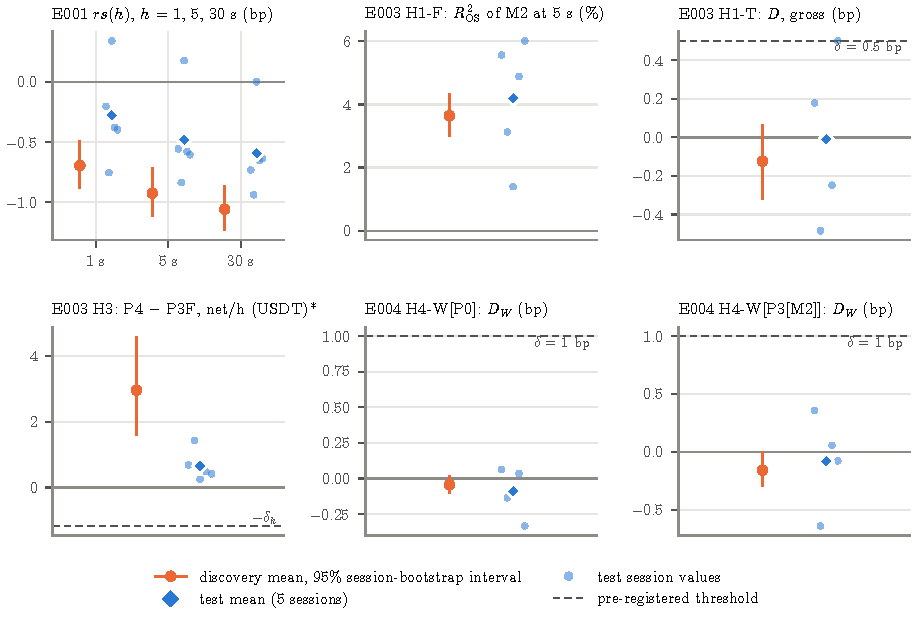
\includegraphics[width=\linewidth]{figures/fig5_holdout.pdf}
  \caption{Selected pre-registered checks (E001 realized spreads, H1-F, H1-T, the net-per-hour component of H3, and
  H4-W), discovery against held-out test. Orange: discovery mean and 95\% session-bootstrap
  interval. Blue: the five test sessions and their mean. Dashed lines: pre-registered thresholds. Test intervals are not
  drawn, because the protocol makes no interval decision on five sessions. E001 and H1-F are \obs; H1-T is \mhr{} and
  fee-free; H3 is \mhr{} under the \hyp{} LP tier 4 schedule; H4-W is \mhr{} under a synthetic \stress.}
  \label{fig:holdout}
\end{figure}

These labels must be read with their weights. A clean sweep of point-estimate checks is not the same as a set of
statistically significant replications, for four reasons.
\begin{enumerate}
  \item \textbf{The checks are not independent.} E001's six share one event set and are linked by an identity; H1-T
  depends on H1-F; the two H4-W checks share their windows.
  \item \textbf{Several checks are weak by construction.} E003's three are decided by the sign or side of a mean, which
  a null effect would pass up to half the time. E001's six rules and E004's two H4-W rules add a four-of-five count
  condition, which bounds that probability at 18.75\% under independent sessions and a null whose median sits at the
  threshold. The secondary $y_\mathrm{view}$ confirmation is largely implied by the choice of target.
  \item \textbf{Some confirmations are narrow.} H1-T held by 0.01\bp; E001's one-second realized spread has a descriptive
  interval that includes zero.
  \item \textbf{Magnitudes shrank.} The passive side's realized spread was about half its discovery size, and H3's net
  improvement about a fifth.
\end{enumerate}
What the holdout does show is that no primary check reversed sign out of sample, that the forecast's skill held at a
similar level, and that the forecast-gated rule again showed no material improvement in per-notional fill quality. The unfavourable descriptive results recurred too:
every policy that traded lost money in every held-out session at the attainable fee.

\section{Discussion}\label{sec:discussion}

\paragraph{Why predictability does not become profit.} Three gaps separate a forecast that predicts the mid from a
quote that earns money.

The first is \emph{magnitude}. The five-second forecast has a mean absolute value of about 0.4 to 0.5\bp, roughly one
tick or less, while the spread is one tick and the attainable maker fee is 10\bp. Even a perfectly calibrated forecast of
this size cannot clear the fee, which is why the fee-aware policies never quote.

The second is \emph{selection}. A passive quote is filled when another trader chooses to trade against it. The markouts in
E001 show that this choice is, on average, informed: the mid moves against the filled side within a second. A forecast
that withdraws quotes ahead of predicted moves need not escape this, because the trades that still reach the quote tend to
be the ones the forecast did not anticipate. In the language of \citet{glosten1985}, the quoter faces a mixture of informed
and uninformed flow whatever it predicts; in the language of \citet{copeland1983}, a resting quote is an option, and the
forecast changes which options are written, not who exercises them. H1-T's near-zero $D$ in both samples is consistent with this argument for
the rules tested, although it cannot exclude a small improvement.

The third is \emph{cost structure}. Fees are charged on notional, so a policy that trades less pays less. When the gross
edge per unit of notional is negative and roughly the same across policies, any reduction in participation reduces
losses. Hourly profit comparisons therefore conflate two effects that the design separates: participation, which every
rule can change, and fill quality, which only a genuine edge can. The per-notional placebo contrasts in E003 and E004
address the second and, for the rules tested, find no material effect at the resolution that ten discovery and five
held-out sessions allow.

\paragraph{Relation to theory and practice.} None of this contradicts the models of optimal market making, which show
how quotes should respond to inventory and signals \emph{given} fill intensities and fees
\citep{avellaneda2008,gueant2013,cartea2018}. It shows that, on this market, at an attainable fee and with a replay in
which the historical stream decides which trades reach the touch, the conditions under which a short-horizon signal adds execution value were not met.
The empirical literature points to what those conditions involve: relative speed \citep{baron2019}, queue position, whose
value can rival the spread \citep{moallemi2017}, and fee terms. Even a successful high-frequency market maker earns the
spread while losing on inventory \citep{menkveld2013}. Our simulated participant has no speed advantage beyond a bracket of
latencies, always joins the back of the queue, and pays the retail fee. The result is consistent with the view that the
revenue from supplying liquidity accrues to participants with structural advantages; it does not establish that market
making is unprofitable for them. It also agrees with live evidence from a Binance perpetual, where maker fill probability
and post-fill returns are negatively related and imbalance-based quoting loses money net of fees
\citep{albers2025dilemma}: two different methods, on two different contracts, point the same way.

\paragraph{Information robustness.} E004's finding of no material deterioration runs against the intuition, and against E004's own specification,
that stale quotes are picked off \citep{foucault2003,foucault2017,budish2015}. Two features of the design explain part of
it. The participant's quotes were withdrawn or left resting at the touch, and when the book moved, quotes left behind by
the move were simply not filled, while quotes the move ran into showed no material deterioration in fill quality under
the 1\bp{} threshold. And the
degradation was synthetic: drops occurred at a stress rate far above the observed reconnect rate, independently of the
market, and did not affect order entry or acknowledgements. A participant whose information fails exactly when the
market moves, or whose order channel is also delayed, could fare differently. In E002, lower latency added fills that
were slightly more adverse per unit of notional (about 0.2\bp), which suggests the extra fills arrive in fast-moving
conditions; we do not test this.

\paragraph{What is established, what we add, and what is open.} \emph{Established before this paper:} liquidity suppliers
face adverse selection; order-book imbalance predicts short-horizon price changes; fees and speed shape the profitability
of liquidity provision; backtests that select among many variants overstate performance; and, from a live experiment
reported as a preprint, maker fills on a Binance perpetual are negatively selected and naive quoting loses even with a
rebate \citep{albers2025dilemma}. \emph{Our empirical
contribution:} on one crypto market, with pre-registered rules and a sealed holdout, we measure each link in the chain
from observed adverse selection to after-cost outcomes, find that, for the forecast-gated rules tested, the forecast's
economic effect operated through participation, with no material improvement in fill quality, show that plausible execution assumptions are second order to fees, and report
the holdout in full, weak labels included. \emph{Open:} whether a policy that models selection conditional on being
filled, rather than the unconditional mid move, could recover a per-fill edge; whether queue-position-aware strategies
change the picture; how results move with venue, instrument and attainable fee tiers; and whether the conclusions hold
on a longer and contiguous holdout than five first-of-month days.

\section{Limitations}\label{sec:limits}

We state the limitations that bound these conclusions, in rough order of importance.

\paragraph{A five-session holdout.} Five sessions give little statistical power. The protocol therefore uses
point-estimate rules whose evidential weight is low and stated in advance (Section~\ref{sec:inference}). A label of
\emph{confirmed} means that a discovery decision did not reverse on five later days; it is not a significance test.
All twenty sessions are first-of-month days, which may not represent other days.

\paragraph{Uneven episode structure.} Held-out valid hours are balanced across sessions, but 2026-06-01 contributes
fourteen of the twenty episodes. Each episode restarts flat, after a sixty-second warm-up, and ends with a liquidation,
so that session carries more episode boundaries than the others. Sessions are equally weighted, so this affects the
composition of one session's value rather than its weight; we did not examine it further, because any such analysis
would be an exploratory reanalysis of the holdout.

\paragraph{Different fitting on the two sides.} Discovery forecasts and fitted quantities are walk-forward: session $k$
uses sessions before it, so early evaluation sessions use as few as five training sessions. The holdout uses models fitted
once on all fifteen discovery sessions. Held-out skill is therefore not directly comparable with the walk-forward
average, and part of the difference between them may reflect training-sample size.

\paragraph{Regime shift.} The holdout's relative tick (0.85 to 1.38\bp) is coarser than most of discovery (0.46 to
1.20\bp), and pre-event book states were older. Basis-point thresholds were not rescaled. Smaller held-out realized spreads
are consistent with this shift; we did not test whether it explains them.

\paragraph{Not blind.} The instrument, sample and splits were chosen with knowledge of all twenty days' data-quality
metadata, though not their outcomes. Each later experiment was designed with knowledge of earlier discovery results, which
it disclosed. During a review of the evaluation protocol, two rows of BTCUSDT acceptance metadata dated 2026-06-01
were displayed; no SOLUSDT test-day row, test-session data file or outcome was read, and we do not regard the exposure as
evidence of leakage.

\paragraph{Test rules written after discovery.} Several held-out rules and test forms were written after the discovery
results were known, though before any test outcome existed: E001's confirmation rule, the four-of-five definedness rule,
the literal reading of H1-T and its carried gates, the fixed $\delta_h$, the test forms of E004's qualifiers, and the
combined rule for the $y_\mathrm{view}$ row. They are disclosed in the frozen protocol.

\paragraph{Modeled execution.} Every policy result is a replay. Our orders have no market impact, queue position is
inferred rather than observed, hidden and intra-batch flows are invisible, and the latency brackets are calibrations, not
measurements of a real participant. Hypothetical executions built from transaction data can be poor proxies for actual
limit-order executions \citep{lo2002}, and live experiments find that realised taker outcomes fall short of what the book at
submission implies \citep{albers2025latency}. The three fill models bracket assumptions; with reactive policies they are not
guaranteed bounds on outcomes. Fees for March to October 2025 are inferred from identical published values on both sides
of that interval.

\paragraph{Synthetic stresses and hypothetical fees.} E004's degradations are synthetic, at stress levels far above
observed rates and independent of market conditions. H3 is tested only under a rebate tier this project cannot reach,
and every LP-programme taker rate is assumed. The fee schedules are accounting overlays on fixed fills: in a market where
fees changed, quotes and order choices would change too \citep{malinova2015}.

\paragraph{Selection by the future path.} Valid windows end when the book leaves the region proven by its last snapshot,
which tends to happen after large moves. Requiring outcomes inside the window removes events according to what the price
did after them. This affects E001's horizons and the forecast targets, and it is disclosed rather than corrected.

\paragraph{Fixed, simple policies.} The policies are a-priori rules, not optimised strategies, and the forecasts are
linear. Negative results speak to these rules. P3's gate ignores selection conditional on being filled, and the fee gates
of P3F and P4 overstate a rational quoter's participation.

\paragraph{One market and venue.} All results concern Binance spot SOLUSDT on a free data sample.

\paragraph{Procedural qualifications.} The protocol allowed up to three technical attempts; one was used. Input
integrity was verified at fixed points of the evaluation rather than continuously. Any further analysis of the held-out
sessions is post hoc and exploratory.

\section{Conclusion}\label{sec:conclusion}

On Binance spot SOLUSDT, short-horizon order-book signals predict price changes out of sample, and liquidity resting at the
best quotes is adversely selected. In a fill-level replay, the forecast-gated rules we tested showed no material improvement in
per-notional fill quality relative to a placebo, and their lower losses came mainly from trading less; five held-out
sessions cannot rule out a small improvement. At the only fee tier attainable to a participant like us, every policy that
trades loses money in every session, execution assumptions move results by less than a basis point, and the rational
decision is not to participate. Under a hypothetical rebate tier, inventory controls reduce risk without creating profit;
at the attainable fee the policies that carry them do not trade. Under synthetic interruptions of the participant's market
data, fill quality showed no material deterioration under the pre-registered threshold. In a one-time evaluation on five
sealed sessions, under rules frozen before any held-out outcome was computed, every primary check met its point-estimate rule (E001 6 of 6, E003 3 of 3,
E004 2 of 2), several of them weakly or narrowly, and the reported-only results, including the losses of every policy
that trades, were consistent with discovery. The paradox in
the title is therefore not that prediction fails, but that prediction, at this scale and cost, is the wrong currency: a
passive quoter is paid for supplying liquidity, and it is charged for being selected against.

\section*{Data and code availability}
The market data are free public samples, Tardis's first-of-month captures of Binance's depth stream and Binance's public
trade archive, and are not redistributed. The experiment specifications, the frozen evaluation protocol, the code and
the result files behind every table and figure are archived in the project's version-controlled repository. A separate
reproducibility supplement lists, for each result, its specification, output and version identifier, the software
environment, and the checks performed before the held-out evaluation.

\section*{Disclosure}
This research was self-funded and used only free public data and local computation. It involved no live trading.

\bibliographystyle{plainnat}
\bibliography{references}

\end{document}
